\chapter{Introducción}
En el transcurso de los últimos años, es decir, desde la década de los 2000 en adelante, ha habido un aumento considerable en el uso de tecnologías renovables para la obtención de energía eléctrica a lo largo de todo el planeta. El consenso internacional de avanzar en pos de un desarrollo sustentable para la humanidad y que esta, a la vez, sea amigable con el resto de las especies y los recursos naturales, da la intuición de que es la manera correcta para progresar y por lo tanto se debe desplegar la mayor cantidad de capital humano para que estas tecnologías continúen en un proceso de mejora continua y se asegure el bienestar de toda la sociedad.

De manera mas concreta, esto se está llevando a cabo a través del uso e implementación de las Energías Renovables No Convencionales (en adelante ERNC) y que corresponden a la energía solar, la energía hidráulica, la mareomotriz, undimotriz, geotérmica, biomasa y eólica. Para el alcance de este trabajo de tesis, se está interesado en la energía eólica, que es aquella energía que se extrae del viento en movimiento.

El recurso viento posee la particularidad de ser extremadamente variable en todo su espectro de escalas temporales y espaciales, es decir, presenta fenómenos cíclicos distinguibles en cada una de estas escalas. Desde los cambios que tiene en la escala climática (ciclos planetarios, cambio climático) hasta la microescala (turbulencia, interacción con el terreno) y por ende la generación de energía a partir de este es indistintamente variable. 
 

%Este hecho sustenta la necesidad de tener predicciones para la rapidez del viento lo mas cercanas a la realidad que se puedan, ya que variaciones en la potencia que puede generar un parque eólico puede significar la no rentabilidad económica de este, entre otros problemas como mantenciones correctivas o fallas en la planificación de la mantención preventiva de las turbinas y la aparición esfuerzos no deseados en el aspa.

En la práctica existe un conflicto permanente en que las zonas con mayor potencial eólico (i.e. aquellos lugares donde estadísticamente se tienen velocidades del viento lo suficientemente altas para que sea conveniente generar energía de estos), son aquellas con terreno complejo, o sea, terreno con topografía no regular como las costas o montañas, esto debido a la aceleración que toma el viento al ajustarse a los contornos del suelo. Existe entonces una dicotomía o conflicto entre que los lugares mas aptos para poner parques eólicos, son al mismo tiempo los mas turbulentos y los más difíciles de predecir.

De este modo, surge la necesidad de buscar maneras teóricas y prácticas para tener completamente determinado el comportamiento y la rapidez del viento en su interacción con el terreno complejo y así tener también determinada la potencia eléctrica que se puede generar de esta.

Históricamente, se ha dependido de técnicas estadísticas (describiendo el viento a través de distribuciones de probabilidad) basadas en bases de datos que contienen mediciones del viento a lo largo de varios años. El problema con este acercamiento es que para terreno complejo, en donde el comportamiento del viento es en gran parte no homogéneo, este no refleja el movimiento real ni los fenómenos no lineales (como el desprendimiento de la capa límite o la mezcla turbulenta) dentro de la zona de interés. Aún asi, si se quisiera aplicar estos métodos estadísticos, el volumen de instrumentación necesaria sería inmenso para aplicarlo en zonas localizadas y por lo tanto, los costos asociados serían demasiado altos como para que se pudieran llevar a cabo en todos los lugares en donde se quisieran instalar turbinas.

Se busca entonces aplicar un método indirecto, y aqui es donde se ve atractivo predecir el comportamiento del viento a través de simulaciones numéricas. 

Evidentemente, las simulaciones se encargarán de resolver las ecuaciones que rigen el comportamiento de la atmósfera. Estas ecuaciones son las llamadas ecuaciones primitivas y dan origen a una rama de la meteorología llamada predicción numérica del clima (Numerical Weather Predicción o NWP).

La predicción numérica del clima no es algo que se viene realizando desde hace poco. Las primera simulaciones atmosféricas datan desde el los años 20, en donde Lewis Fry Richardson logró hacer un pronóstico para 6 horas en dos puntos de Europa central. Este cálculo tardó cerca de dos semanas debido a que fueron realizados a mano. No fue hasta la década del 50, con la llegada de los computadores, que este campo pudo desarrollarse mas intensivamente, principalmente gracias al trabajo desarrollado por el grupo de investigación de Carl-Gustav Rosby que logró un pronóstico de 6 horas operativo. Desde aquí en adelante, el avance exponencial de la computación y la sofisticación de las ecuaciones que modelan la atmósfera, han permitido tener pronósticos cada día mas precisos y para ventanas de tiempo cada vez mayores. 

Si bien las ecuaciones que permiten modelar la circulación planetaria de la atmósfera se conocen desde hace décadas, nuestra vida como seres humanos (o por lo menos la mayoría de nosotros) y la vida en general, se confina a una pequeña parte de esta. A esta parte se le denomina capa límite planetaria, y es aquella zona que está influenciada directamente por las condiciones del suelo y que en promedio tiene una altura de 1[km]. Los fenómenos que afectan a la capa límite, como por ejemplo la turbulencia originada por los obstáculos, la trasferencia de calor a la superficie terrestre o el intercambio de humedad con la vegetación, son características únicas de esta pequeña parte de la atmósfera. Por lo tanto la precisión que se tiene para estimar el comportamiento global del viento no es directamente útil para estimar el viento dentro de la capa límite, que es donde, como especie, estamos interesados. 

Entonces, frente a esta latente necesidad de conocer el comportamiento del viento dentro de la capa límite para terreno complejo y aprovechando los avances en capacidad computacional que existen actualmente, es que se plantea el uso de simulaciones multiescala que permitan resolver desde las escalas planetarias hasta las escalas mas pequeñas relevantes para el caso de estudio y así obtener pronósticos fiables para zonas muy localizadas. Estos resultados no solamente serán útiles en términos de generación por energía eólica, si no que también sientan las bases de una manera vanguardista para predecir dispersión de contaminantes, zonas de recirculación, evolución de incendios, entre otros.

\begin{figure}[h]
	\centering
	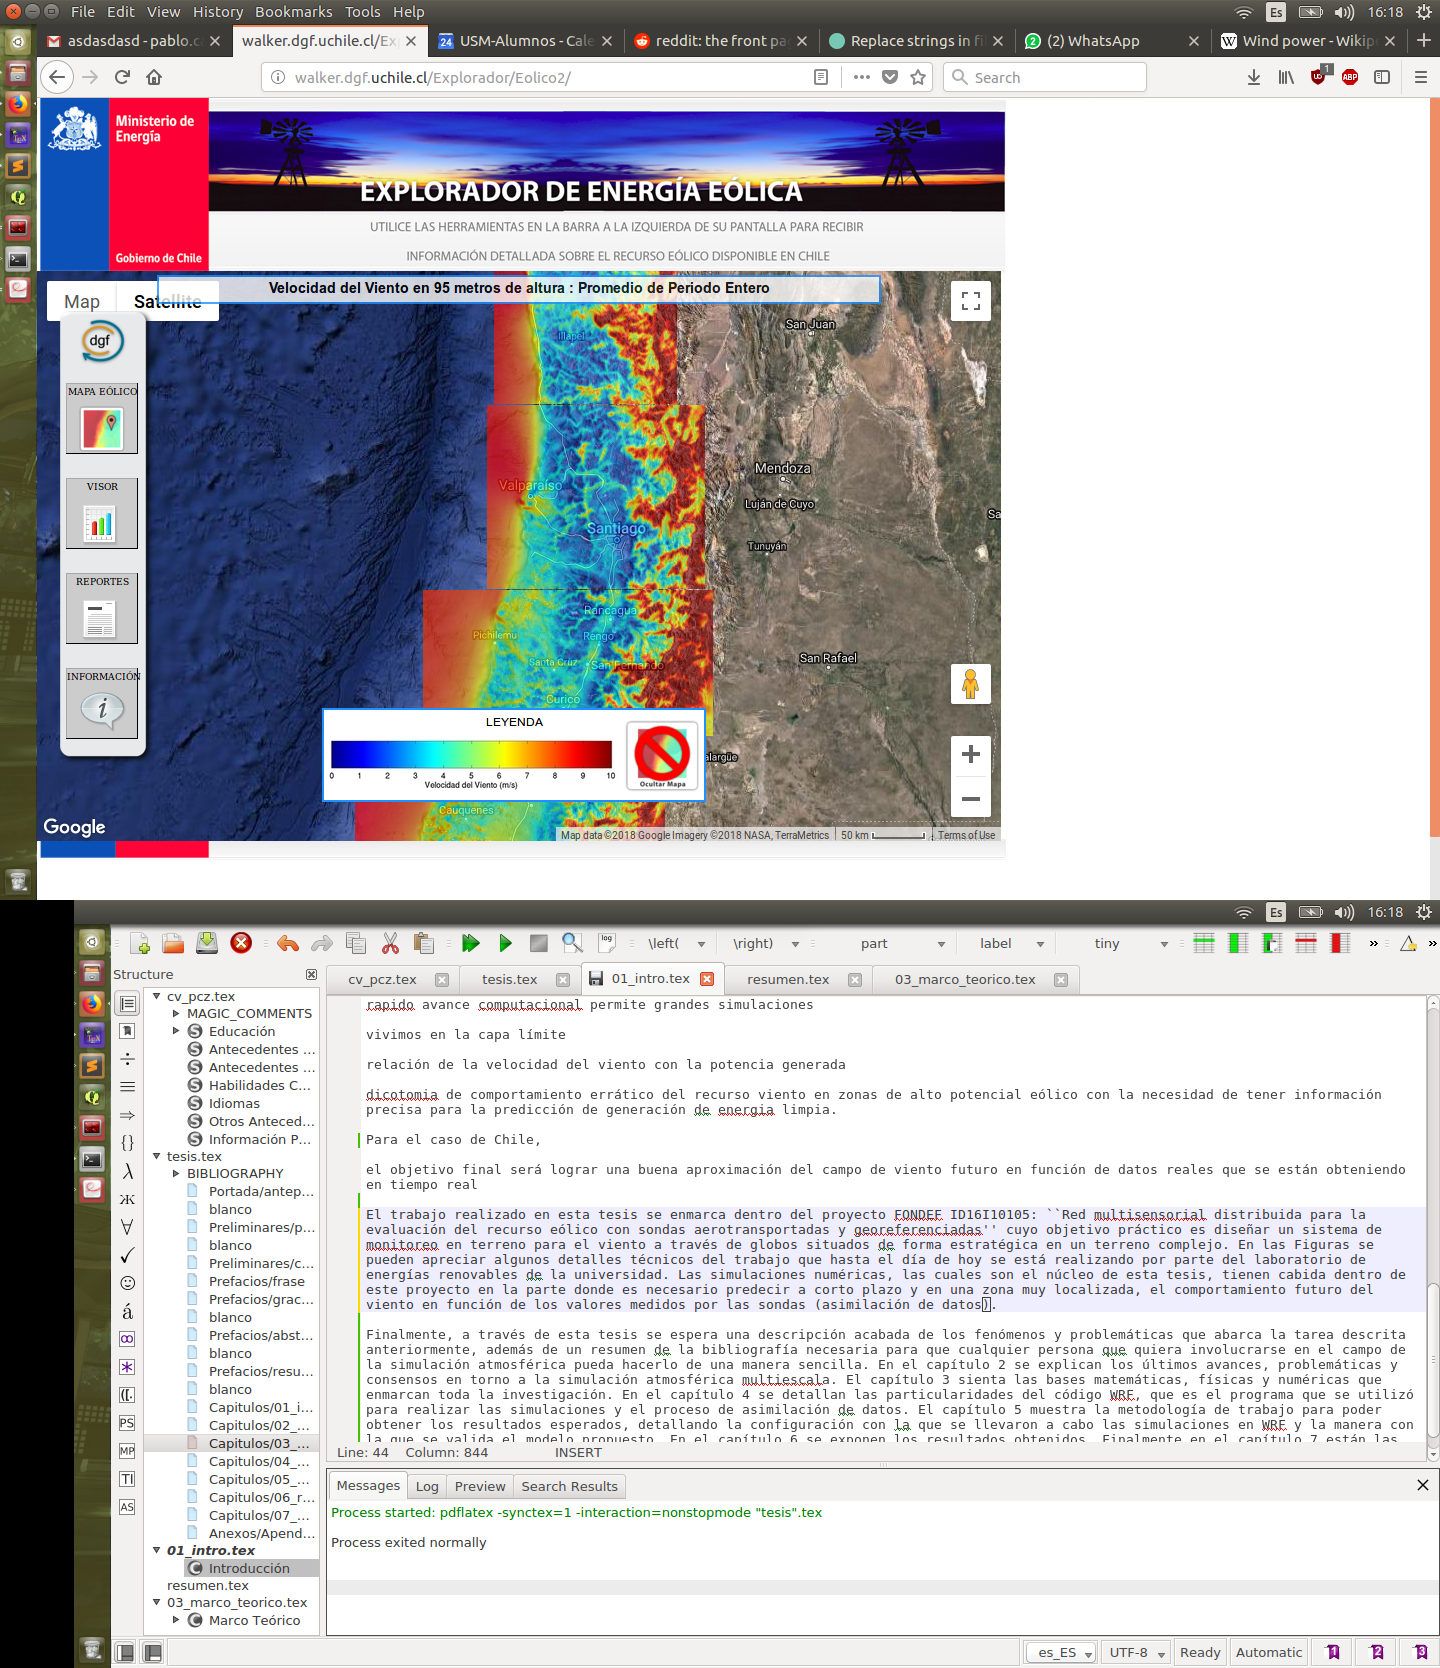
\includegraphics[width=0.9\linewidth,trim={1.4cm 28cm 15cm 3.4cm},clip]{Imagenes/01/explo}
	\caption{Interfaz online del explorador eólico de la Universidad de Chile.}
	\label{fig:01_explorador}
\end{figure}

Aterrizando el tema a una escala mas local, Chile cada año está inaugurando nuevos parques eólicos debido al buen factor de planta que se poseen en ciertas zonas del país (según estudios del Ministerio de Energía en el 2014). Hasta la fecha ya se han instalado mas de 600 turbinas eólicas y la tendencia es a que este número siga aumentando. De la mano de la instalación de nuevas plantas, está la simulación numérica realizada para tener una estimación de la cantidad de energía que se puede llegar a generar. En el 2010, la Universidad de Chile entregó a la comunidad la herramienta online llamada Explorador Eólico, en esta se muestra el potencial eólico que tiene gran parte de Chile, el cual fue simulado a través del software libre WRF. Algunos resultados de esta herramienta se pueden ver en la Figura \ref{fig:01_explorador}.


Si bien esta herramienta ha entregado a Chile información certera y que antes no existía, las simulaciones realizadas para el Explorador Eólico contemplaban mallas numéricas con una resolución horizontal máxima de 1 [km], resolución que no es suficiente para resolver el comportamiento turbulento de microescala, ni para captar efectivamente las variaciones orográficas. El comportamiento del viento a lo largo de una superficie de 1 [km$^2$] puede cambiar mucho, en especial si existe terreno complejo, y por lo tanto la ubicación o no de una turbina eólica requiere un análisis mas detallado del dominio.

El objetivo es entonces buscar una buena aproximación para el campo de viento en la capa límite en terrenos complejos y a alta resolución, a modo de tener un insumo mas realista para efectuar la toma de decisiones en situaciones en donde el viento sea una variable crítica.

Debido a que en la capa límite es donde predominan los fenómenos de mezcla y turbulencia, es acá en donde los modelos presentan la mayoría de sus problemas y desviaciones, y de hecho, el buen comportamiento del un modelo va a depender en gran manera de la habilidad del modelador para ajustar ciertos parámetros arbitrarios del código. 

Como la filosofía de este trabajo es utilizar la información de la manera menos manipulada posible y evitar el ajuste de parámetros, es que se va a buscar la manera de corregir los resultados numéricos a través de un proceso de asimilación de datos utilizando datos reales medidos en terreno.

La asimilación de datos es el proceso matemático mediante el cual se combina información de observaciones y de simulación numérica para obtener el mejor estimador del estado real de la atmósfera en un instante dado. Este proceso se utiliza cotidianamente en modelos globales o sinópticos para entregar la información sobre el clima que se ve día a día en los noticieros.

Para los modelos meteorológicos operativos, el realizar asimilación de datos en la microescala no presenta beneficios, debido a que generalmente la resolución de estos modelos es gruesa en las cercanías de la superficie (la capa límite está pobremente resuelta), lo que se traduce en que la combinación entre observaciones superficiales y resultados numéricos no es fiable.

Sin embargo, y considerando esto como motivación para esta investigación, si se trabaja a resoluciones lo suficientemente altas como para tener información confiable en las cercanías de la superficie, si es posible realizar asimilación de datos en la microescala y por lo tanto mejorar los pronósticos del viento en esta.

El trabajo realizado en esta tesis se enmarca dentro del proyecto FONDEF ID16I10105: ``Red multisensorial distribuida para la evaluación del recurso eólico con sondas aerotransportadas y georeferenciadas'' cuyo objetivo práctico es diseñar un sistema de monitoreo en terreno para el viento a través de globos situados de forma estratégica en un terreno complejo. En las Figuras \ref{fig:01_detalle_fondef} y \ref{fig:01_sonda} se pueden apreciar algunos detalles técnicos del trabajo que hasta el día de hoy se está realizando por parte del Laboratorio de Energías Renovables de la UTFSM. Las simulaciones numéricas, las cuales son el núcleo de esta tesis, tienen cabida dentro de este proyecto en la parte donde es necesario predecir a corto plazo y en una zona muy localizada, el comportamiento futuro del viento en función de los valores medidos por las sondas (proceso de asimilación de datos).

\begin{figure}
	\begin{minipage}{0.5\linewidth}
		\centering
		(a)
	\end{minipage}
	\begin{minipage}{0.5\linewidth}
		\centering
		(b)
	\end{minipage}
	
	\begin{minipage}{0.5\linewidth}
		\centering
		\includegraphics[width=0.9\linewidth,page=3,trim={6cm 12.2cm 6cm 9.5cm},clip]{Imagenes/01/descrp}
	\end{minipage}
	\begin{minipage}{0.5\linewidth}
		\centering
		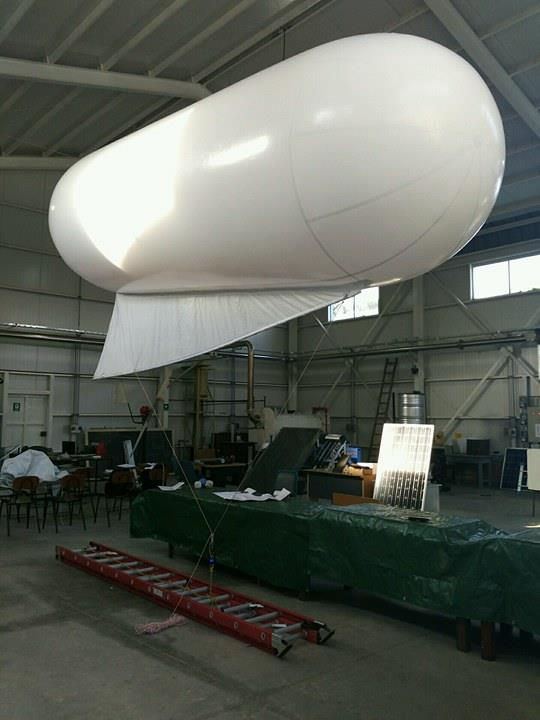
\includegraphics[width=0.7\linewidth,trim={0cm 0cm 0cm 0cm},clip]{Imagenes/01/prototipo}
	\end{minipage}
	\caption{Detalle del proyecto FONDEF ID16I10105. (a) Célula del sistema experimental de medición. (b) Prototipo en el laboratorio.}
	\label{fig:01_detalle_fondef}
\end{figure}


El objetivo final de esta investigación será lograr un sistema robusto que obtenga una buena aproximación del campo de viento futuro en función de datos medidos que se estarán obteniendo en tiempo real, mediante simulaciones numéricas multiescala que se harán, para este caso, con el software libre WRF. La filosofía de simulación, será realizarlas de la manera menos manipulada posible, utilizando bases de datos públicas y evitando la asignación arbitraria de parámetros. La sumatoria de esto tiene como resultado un acercamiento mucho mas vanguardista, y poco investigado, a la predicción eólica en terreno real a alta resolución. 

\begin{figure}[h!]
	\centering
	\includegraphics[width=0.82\linewidth,page=5,trim={3cm 2cm 2.3cm 3cm},clip]{Imagenes/01/descrp}
	\caption{Esquema de la sonda FONDEF ID16I10105.}
	\label{fig:01_sonda}
\end{figure}

Finalmente, a través de esta tesis se espera una descripción acabada de los fenómenos y problemáticas que abarca la tarea descrita anteriormente, además de un resumen de la bibliografía necesaria para que cualquier persona que quiera involucrarse en el campo de la simulación atmosférica pueda hacerlo de una manera sencilla. Como beneficio para la comunidad científica, los resultados obtenidos acá podrán ser utilizados como linea de base o benchmark para cualquier otra simulación futura a alta resolución, pudiendo dar pié a ser un nueva prueba para modelos multiescala.

\section{Caracterización de la Tesis}
\subsection{Hipótesis}

Mejorar la precisión de los pronósticos actuales para el viento a través de simulaciones atmosféricas multiescala de alta resolución en terreno complejo y la incorporación de un esquema de asimilación de datos 4D que vaya alimentando datos al sistema en tiempo real.

\subsection{Objetivos}
\subsubsection{Objetivo Principal}
\begin{itemize*}
	\item Desarrollar un sistema de predicción de viento en terreno complejo de alta resolución en base al código libre WRF que proponga una mejora comparativa con respecto a los modelos existentes a través del uso de la asimilación de datos en la capa límite atmosférica.
\end{itemize*}
\subsubsection{Objetivos Secundarios}
\begin{itemize*}
	\item Acoplar dominios de microescala y mesoescala en las simulaciones numéricas mediante una clausura de turbulencia a través del modelo LES.
	\item Estudiar el uso e incorporación de bases de datos reales de alta resolución para orografía y tipo de uso de suelo en el modelo WRF.
	\item Desarrollar y optimizar códigos relacionados con simulación atmosférica multiescala y asimilación de datos.
	\item Estudiar la influencia de la asimilación de datos en la capa límite considerando un solo punto y multipunto.
	\item Verificar y validar resultados obtenidos con aquellos presentes en el estado del arte y campañas de medición en terrenos reales.
\end{itemize*}

\section{Estructura del Documento}
La estructura de la tesis es la siguiente:
\begin{itemize*}
	\item Cap. 2: Se exponen los últimos avances, problemáticas y consensos en torno a la simulación atmosférica multiescala y asimilación de datos, que son el núcleo del trabajo realizado.
	\item Cap. 3: Sienta las bases conceptuales, matemáticas y físicas sobre las cuales se desarrolla la investigación. Acá se abordan: las leyes fundamentales de los fluidos, la dinámica atmosférica, la turbulencia, la capa límite planetaria, el método de simulación de grandes vórtices (LES) y la asimilación de datos.
	\item Cap. 4: Sienta las bases numéricas, es decir, se explica el funcionamiento del software  libre WRF.
	\item Cap. 5: Muestra la filosofía y configuración de los 4 experimentos realizados: 2 casos para terreno plano (donde uno sirve como validación y el otro analiza la asimilación de datos) y dos casos para terreno complejo (sin y con asimilación). Además, se detalla la metodología para la obtención y presentación de resultados.
	\item Cap. 6: Se presentan los resultados mas relevantes.
	\item Cap. 7: Conclusiones, trabajo futuro y aspectos que quedan abiertos a la mejora.
\end{itemize*}
